\documentclass{report}
\usepackage[spanish]{babel}  % Idioma español
\usepackage{graphicx}       % Para incluir imágenes
\usepackage{float}          % Para controlar la posición de las imágenes
\usepackage{titlesec}       % Para modificar títulos de capítulos
\usepackage{geometry}       % Para ajustar márgenes

% Ajustar márgenes
\geometry{a4paper, margin=2.5cm}

% Configurar capítulos sin la palabra "Capítulo"
\titleformat{\chapter}[display]
  {\normalfont\huge\bfseries}{}{0pt}{\Huge}

% Portada
\begin{document}
\begin{titlepage}
    \centering
    \vfill
    {\Huge\bfseries Ankidyemy}\par
    \vspace{1cm}
    {\LARGE Diseño de Software}\par
    \vfill
\end{titlepage}

% Diagrama Entidad-Relación
\chapter{Diagrama Entidad-Relación}
\begin{figure}[H]
    \centering
    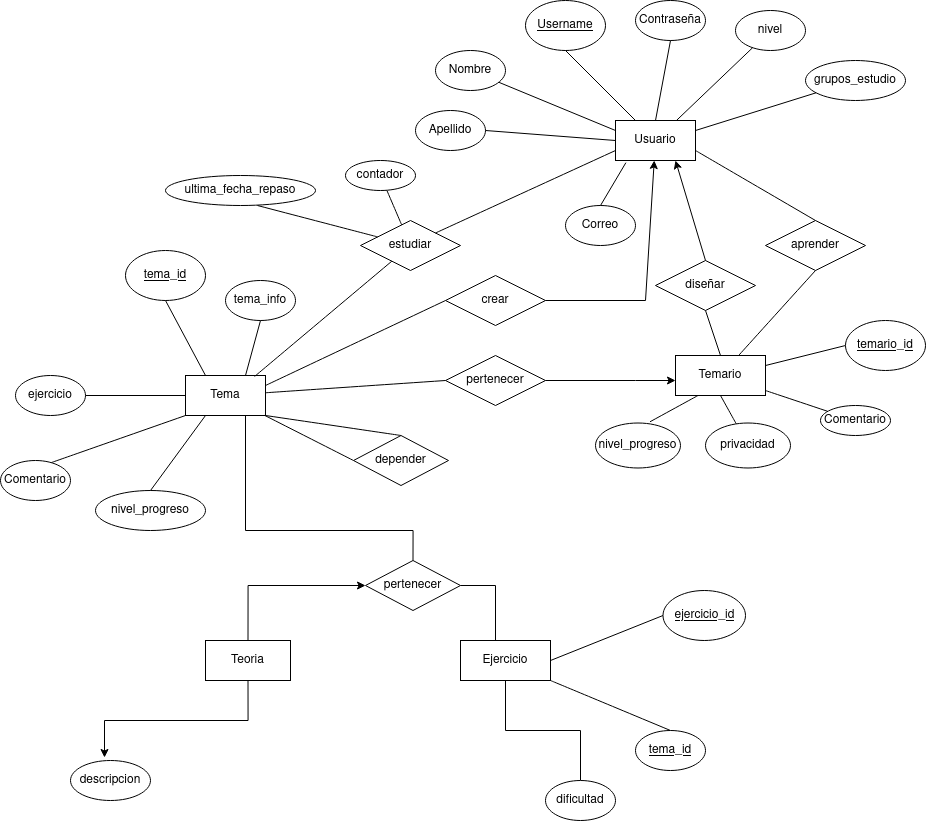
\includegraphics[width=0.8\textwidth]{./Diagramas/Diagrama-ER.png}
    \caption{Diagrama Entidad-Relación del sistema}
    \label{fig:er}
\end{figure}

\section{Explicación del Diagrama}
Las entidades principales de nuestra base de datos son Usuario, Tema y Temario. El ususario se relaciona con los Temas y los Temarios de dos formas distintas, como diseñador o creador de los diferentes temas y ejercicios por temario, y como alumno de los temarios.

% Módulos
\chapter{Módulos}

\section{Módulo 1: BD Administrador}
Este módulo pensamos que ayude administrar la conexión de base de datos, así como proveer las operaciones básicas de CRUD a los demás módulos del sistema.

\begin{figure}[H]
    \centering
    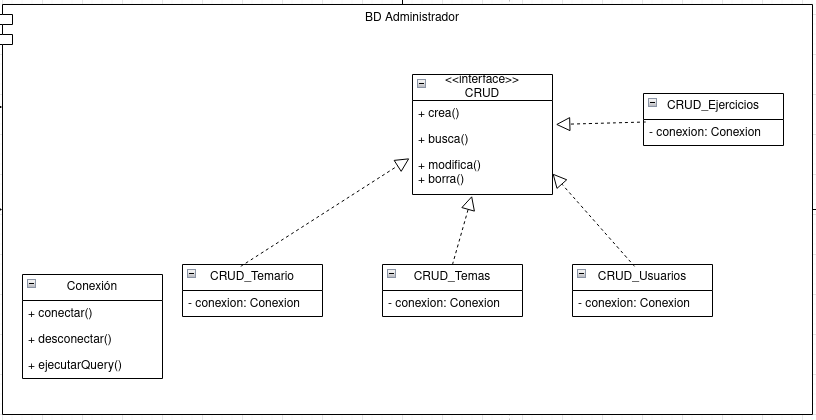
\includegraphics[width=0.8\textwidth]{./Diagramas/Modulo1.png}
    \caption{Diagrama UML del Módulo 1}
\end{figure}

\section{Módulo 2: Autenticación}
EL módulo se encargaría de hacer el inicio de sesión, verificando los datos del usuario e iniciando la sesión.

\begin{figure}[H]
    \centering
    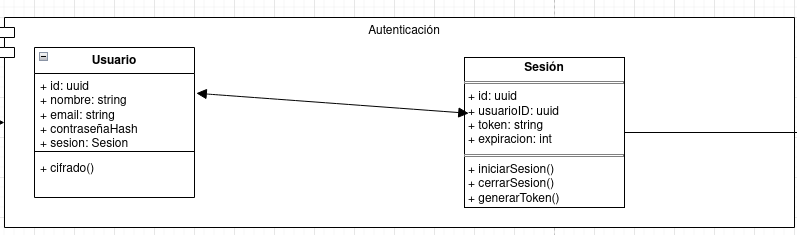
\includegraphics[width=0.8\textwidth]{./Diagramas/Modulo2.png}
    \caption{Diagrama UML del Módulo 2}
\end{figure}

\section{Módulo 3: ED\_Temas y Jerarquía}
Se encarga de proporcionar la estructura de datos de gráfica de conocimientos, además de dar un gestor que permita transmitir los cambios en la sesión a la base de datos.

\begin{figure}[H]
    \centering
    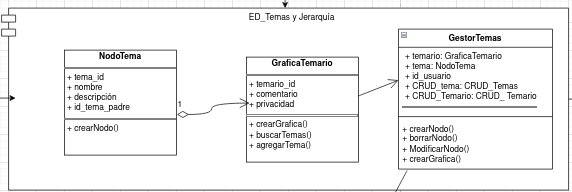
\includegraphics[width=0.8\textwidth]{./Diagramas/Modulo3.png}
    \caption{Diagrama UML del Módulo 3}
\end{figure}

\section{Módulo 4: Sesión de Estudio}
Este módulo es el principal en el modo de estudio, el objeto SesiónRevisión a través del Elector\_Tema regresa el ejercicio a realizar utilizando los parámetros de avance en el tema y fecha de última revisión basándose en el concepto de repetición espaciada.

\begin{figure}[H]
    \centering
    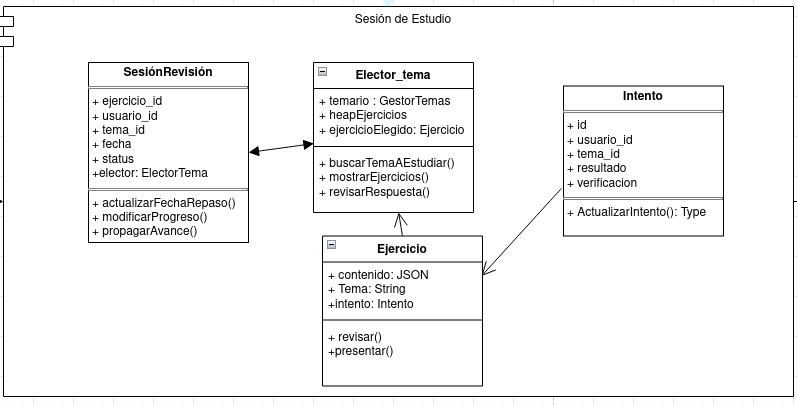
\includegraphics[width=0.8\textwidth]{./Diagramas/Modulo4.png}
    \caption{Diagrama UML del Módulo 4}
\end{figure}

\section{Módulo 5: Compartir}
El módulo se encargará a traves del objeto Temario de crear y compartir los Temarios.

\begin{figure}[H]
    \centering
    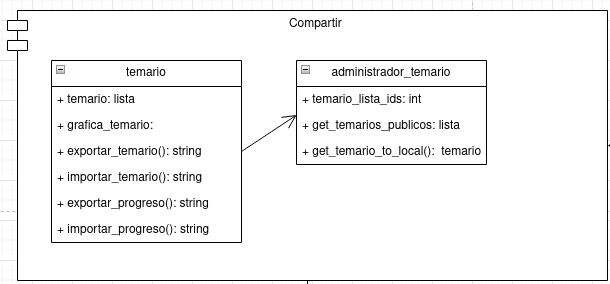
\includegraphics[width=0.8\textwidth]{./Diagramas/Modulo6.png}
    \caption{Diagrama UML del Módulo 5}
\end{figure}

\section{Módulo 6: Main}
Utilizando la librería Gin que proporciona Go para establecer un servidor sería el punto de entrada para el backend.

\begin{figure}[H]
    \centering
    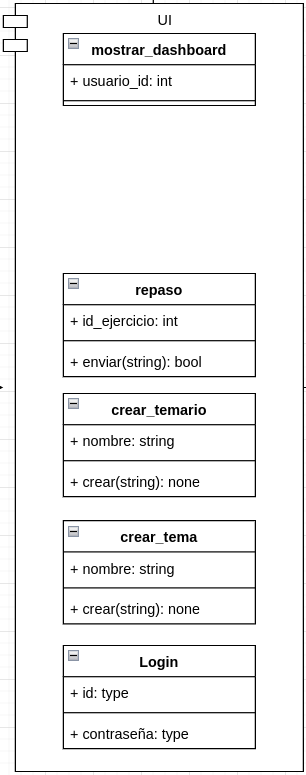
\includegraphics[width=0.4\textwidth]{./Diagramas/Modulo7.png}
    \caption{Diagrama UML del Módulo 6}
\end{figure}

\section{Módulo 7: UI}
Es el módulo de la interfaz gráfica.

\begin{figure}[H]
    \centering
    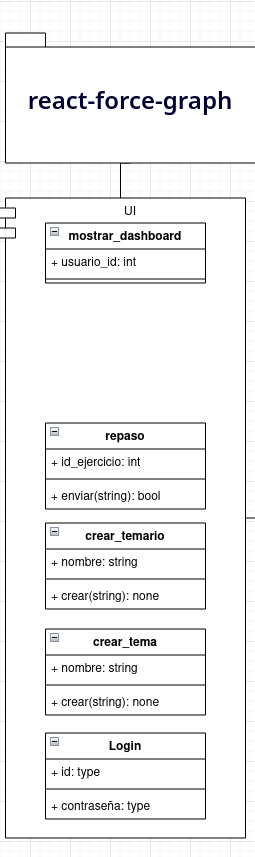
\includegraphics[width=0.15\textwidth]{./Diagramas/Modulo8.png}
    \caption{Diagrama UML del Módulo 8}
\end{figure}
\section{Relación entre módulos}

\begin{figure}[H]
    \centering
    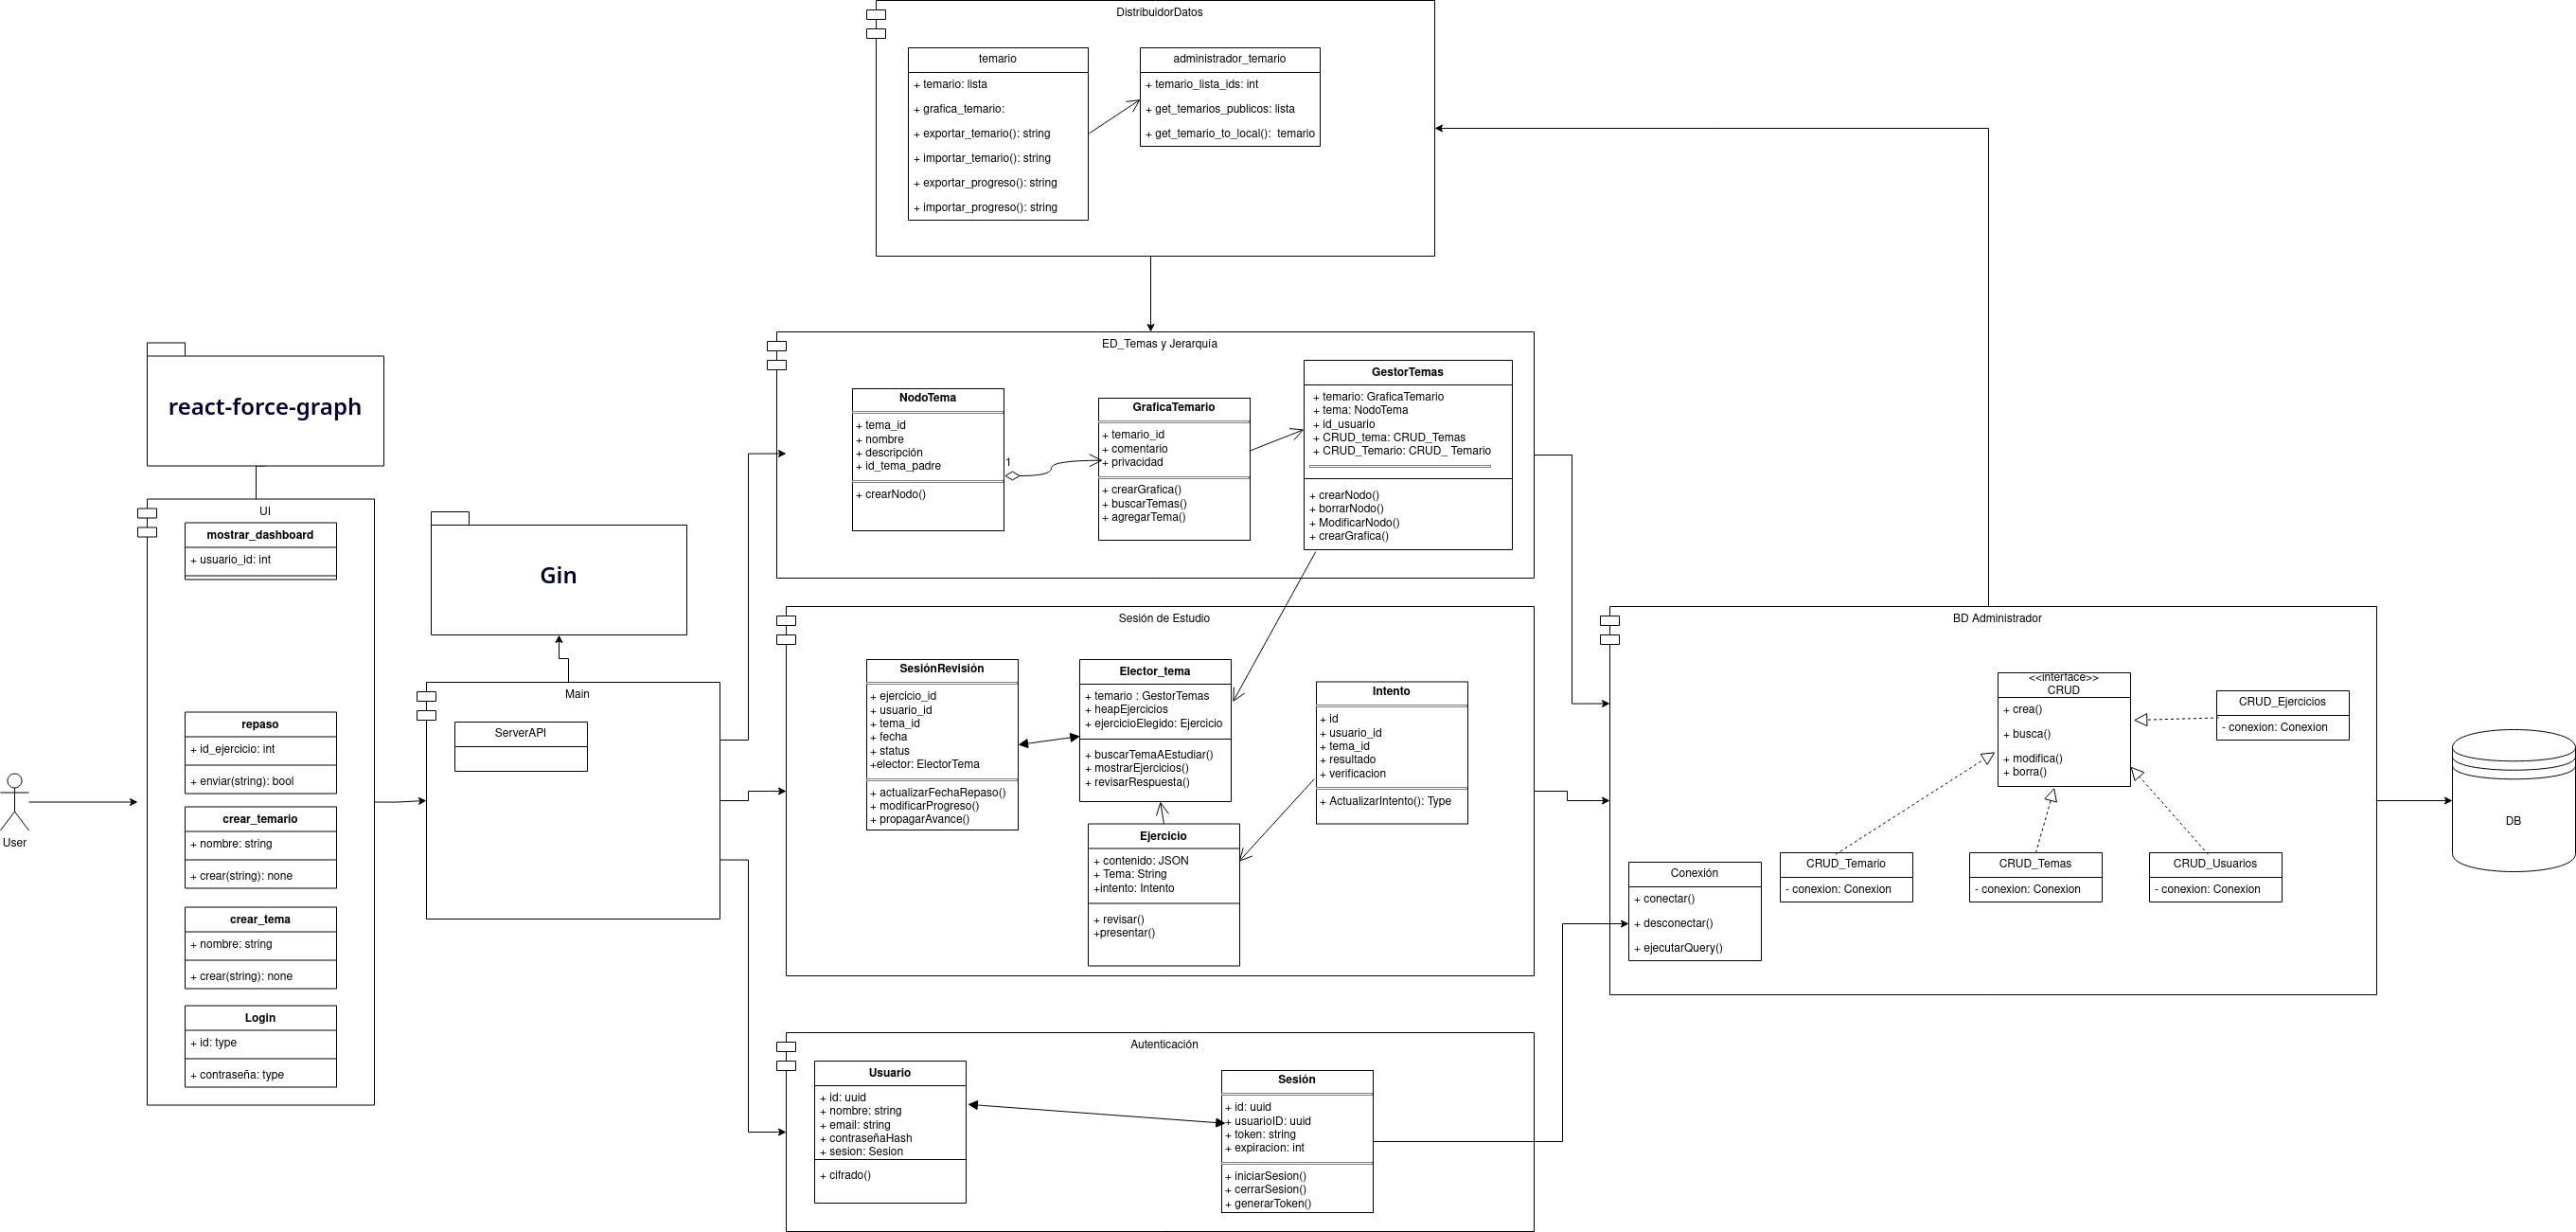
\includegraphics[width=1.55\textwidth, angle=270]{./Diagramas/Diagrama-Modulos.png}
    \caption{Diagrama general de la relación entre módulos}
\end{figure}

% Wireframes
\chapter{Wireframes}

\begin{figure}[H]
    \centering
    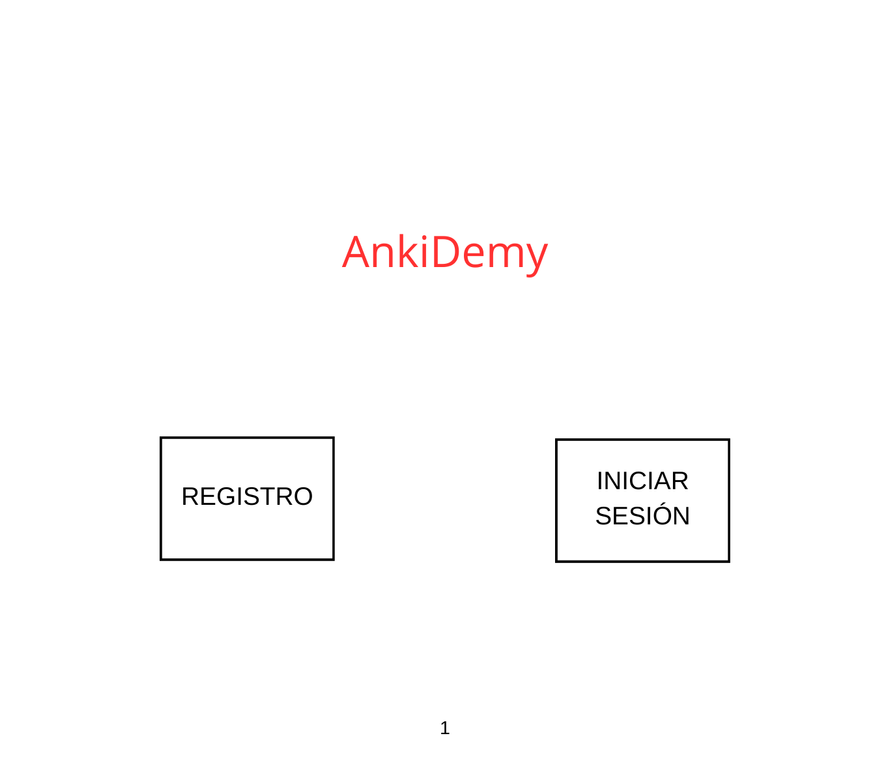
\includegraphics[width=0.8\textwidth]{./Diagramas/1.png}
    \caption{Ejemplo de wireframe del sistema}
\end{figure}

\end{document}
